\section{The crest construction in detail}\label{app:construction}

\subsection{Ground and mountain area}\label{sec:data}

The elevations are delivered in tiles of $25\times25$~km. A massif is the set of departments of Appendix~\ref{app:params}; its mosaic covers the
bounding box of their tiles, \CgAlpsCells{} million cells in the Alps and \CgPyrCells{} million in the Pyrenees. The tiles of neighbouring departments that fall in the box are read, so that water can leave a department;
outside France there is no data.

The mountain area follows the classes of UNEP-WCMC (Kapos et al.\ 2000~\cite{kapos}), evaluated on 1~km cells from the model itself. For a cell of $40\times40$ model cells let $\bar z$ be its mean elevation, $\sigma$ the
slope of the 1~km grid and $\Delta z$ the local elevation range, the difference between the highest and the lowest $\bar z$ within \CgPMountainRadius~km. A cell is mountain if
\begin{equation}
  \begin{aligned}
  &\bar z \ge 2500~\mathrm{m},\ \text{or}\\
  &\bar z \ge 1500~\mathrm{m}\text{ and }\sigma \ge 2^\circ,\ \text{or}\\
  &\bar z \ge 1000~\mathrm{m}\text{ and }(\sigma \ge 5^\circ\text{ or }\Delta z > \CgPMountainRange~\mathrm{m}),\ \text{or}\\
  &\bar z \ge 300~\mathrm{m}\text{ and }\Delta z > \CgPMountainRange~\mathrm{m}.
  \end{aligned}
  \label{eq:kapos}
\end{equation}
Enclosed pieces of at most \CgPBasinKm~km$^2$ that are not mountain, surrounded by mountain, are added, and the largest connected piece is kept. The area is computed on the tiles
of the departments themselves, and the cells of neighbouring tiles count as no data. A massif is the set of the departments of its \emph{loi Montagne} massif; taking the neighbouring tiles
as data would add the mountains of neighbouring departments that touch it. Figure~\ref{fig:map} shows the area and the crest curves of both massifs.

\begin{figure}
\centering
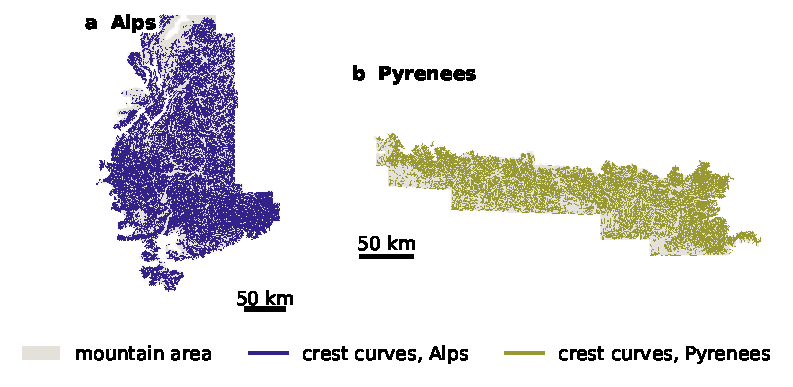
\includegraphics[width=\textwidth]{figures/map.pdf}
\caption{The crest curves cover the mountain area of both massifs. Mountain area in grey, crest curves of the Alps (indigo) and the Pyrenees (olive); the curves are drawn every 10th point.}
\label{fig:map}
\end{figure}

\subsection{Crests as divides}\label{sec:divides}

\paragraph{Valleys and links.} The elevations are depression-filled by a priority flood, starting from the cells at the border of the mosaic and next to cells without data. Every cell $c$ drains to its steepest lower
neighbour among the eight around it; cells of a filled depression or of a flat drain to the cell that reached them. The drainage area $A(c)$ is the number of cells that drain through $c$ times
625~m$^2$. The valleys are the cells with $A(c)\ge A_{\min}=\CgPValley$~km$^2$ (\CgPValleyCells{} cells), cut into links at the confluences. Let $\ell(c)$ be the link into which $c$ drains, undefined if
$c$ drains to the edge of the data without meeting a valley.

\paragraph{Divide sides.} Two neighbouring cells $a$ and $b$ are on a divide if $\ell(a)\ne\ell(b)$, both defined, and neither link is downstream of the other. Divides are thus continuous through summits
and cols. The divide is the set of the shared sides; they form a planar network on the cell corners.

\paragraph{Two tests.} The cross-section test is Eq.~\eqref{eq:xsec}; where the ground is missing the side passes. The second test is on the height above the streams. Let $z_s(c)$ be the filled elevation of the valley cell where $c$
enters the valley network and
\begin{equation}
  h(c)=z(c)-z_s(c),\qquad h(a)\ge h_{\min},\quad h(b)\ge h_{\min},\quad h_{\min}=\CgPHandMin~\mathrm{m}.
  \label{eq:hand}
\end{equation}
A valley cell has $h=0$; a cell in a filled depression has $h<0$. Figure~\ref{fig:divides} shows both tests. In the Alps \CgAlpsSides{} sides pass both and \CgAlpsFlat{} fail only the cross-section; in the Pyrenees
\CgPyrSides{} and \CgPyrFlat. The sides that fail only the cross-section are candidates to bridge flat stretches.

\begin{figure}
\centering
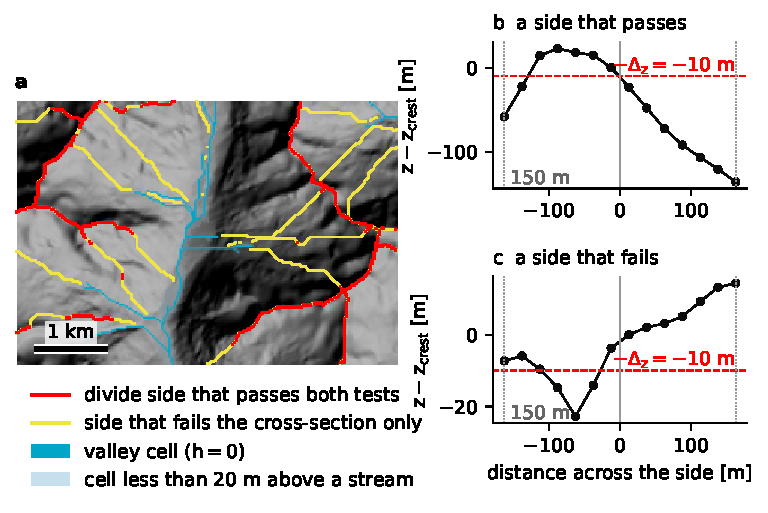
\includegraphics[width=\textwidth]{figures/divides.pdf}
\caption{A divide side is a crest if the ground falls away on both sides. \textbf{a}~Divide sides on the hillshade of a part of the Écrins. \textbf{b}~Elevation $z-z_{\mathrm{crest}}$ along the axis through the two cells of a
side that passes the cross-section: dotted lines mark $n$ cells ($\CgPXsecM$~m) from the side and the dashed red line the drop $-\Delta_z$ the ground must reach there. \textbf{c}~The same for a side that fails.}
\label{fig:divides}
\end{figure}

\subsection{From the network to curves}\label{sec:curves}

\begin{enumerate}[nosep]
  \item \textbf{Bridges.} A ridge that flattens fails the cross-section over a stretch. The sides that pass the height test but fail the cross-section are candidates; a stretch of at most \CgPBridgeSides{} sides
        (\CgPBridgeM~m) that joins the network at two or more places is added, after removing the candidate spurs that touch it once. There are \CgAlpsBridged{} such sides in the Alps and \CgPyrBridged{} in the Pyrenees.
  \item \textbf{Pruning.} Dead ends shorter than \CgPPruneSides{} sides (\CgPPruneM~m) are removed, repeatedly.
  \item \textbf{Strokes.} At a junction of three or four branches a curve goes on along the straightest continuation. Let $u_i$ be the unit vector from the junction to the point of branch $i$ at \CgPDirectionM~m along it.
        The deflection between two branches is $\theta_{ij}=\pi-\angle(u_i,u_j)$. The branches are paired from the smallest $\theta_{ij}$ up, each branch once, and a pair is kept if $\theta_{ij}\le\CgPDeflection^\circ$. A paired branch
        continues the curve; an unpaired branch starts a curve of its own.
  \item \textbf{Spline and resampling.} The sides of a curve make a staircase of 25~m steps. A smoothing spline $f(t)$ through the corners, with $t$ the arc length along the staircase, minimizes
        $\sum_i|f(t_i)-r_i|^2+\lambda\int|f''|^2\,\mathrm{d}t$ with $\lambda=(L_s/2\pi)^4$ and $L_s=\CgPSmooth$~m, so that waves shorter than $L_s$ are removed. The curve is then resampled every $\Delta s=\CgPStep$~m of arc length.
        A cut-off of four cells is the scale below which the shape of a curve is set by the grid, which is also where the fit of $\Hgeo$ starts: the two scales are one choice.
  \item \textbf{Selection.} Curves shorter than \CgPMinLengthKm~km are dropped, and a curve is kept if at least \CgPMaskShare\% of it lies in the mountain area. A curve is flagged as reaching the edge of the data if one of its
        corners is within \CgPEdgeCells{} cells (\CgPEdgeM~m) of a cell without data.
\end{enumerate}

\begin{figure}
\centering
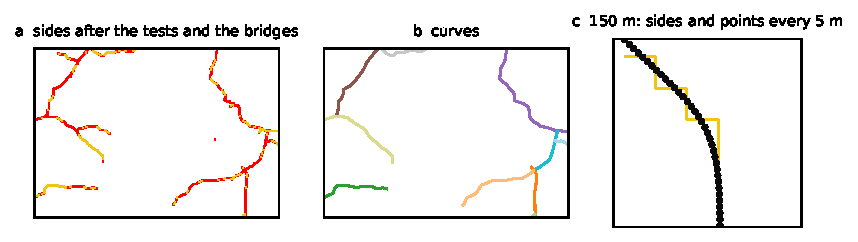
\includegraphics[width=\textwidth]{figures/curves.pdf}
\caption{Sides that pass the tests become smooth curves, which are sampled every $\Delta s$. \textbf{a}~Cell sides of the tests (red) and bridged stretches (orange) under the smoothed curve (indigo) on a hillshade; the rectangle is the window
of b. \textbf{b}~Detail of 150~m: the staircase of cell sides, the curve and its points every $\Delta s$.}
\label{fig:curves}
\end{figure}

\subsection{Joins}\label{sec:joins}

From every dead end of a curve, at point $p$, we look for a straight join to another piece of the crest network with these rules:
\begin{itemize}[nosep]
  \item the target $q$ is on a curve of another component, at distance $|q-p|\le\CgPJoinM$~m;
  \item $q$ lies within $\CgPCone^\circ$ of the direction $u$ in which the curve runs out, the unit vector from the point \CgPRunout~m back along the curve to $p$: $u\cdot(q-p)\ge|q-p|\cos\CgPCone^\circ$;
  \item if a dead end of the target curve lies within \CgPSnap~m of $q$, the join goes to that dead end;
  \item up to \CgPJoinComponents{} other components are tried per dead end;
  \item \textbf{the join never crosses a valley.} Let $C(p,q)$ be the set of all model cells that the segment $pq$ touches, corners included. The join is accepted only if
        \begin{equation}
          \min_{c\in C(p,q)} h(c)\ \ge\ h_{\min}=\CgPHandMin~\mathrm{m},
          \label{eq:joincells}
        \end{equation}
        with $h$ of Eq.~\eqref{eq:hand}. A stream cell has $h=0$ and a cell that drains to no valley has no $h$, so both block the join.
\end{itemize}
Joins are made shortest first; a dead end takes part in at most one, and a join is never made inside a component, so the pieces grow into trees.

\paragraph{Why every cell.} A valley floor is a few cells wide and a stream is one cell. A test on points sampled along the line can step over the corner between two diagonal stream cells and let the join through; the set $C(p,q)$ cannot.
Two tests of \code{test\_joined.py} fix this: two crests separated by a one-cell stream are not joined, nor across a diagonal stream, while two crests across a flat col 25~m above the streams are. After the run every join was checked again
on a sampling every 0.25~m: \CgAlpsJoinsLow{} of the \CgAlpsJoins{} Alps joins and \CgPyrJoinsLow{} of the \CgPyrJoins{} Pyrenees joins touch a cell below $h_{\min}$. Figure~\ref{fig:joins} shows joins on the hillshade: none enters a
green stream cell or a light blue cell, and several run beside a valley and stop short of it.

\begin{figure}
\centering
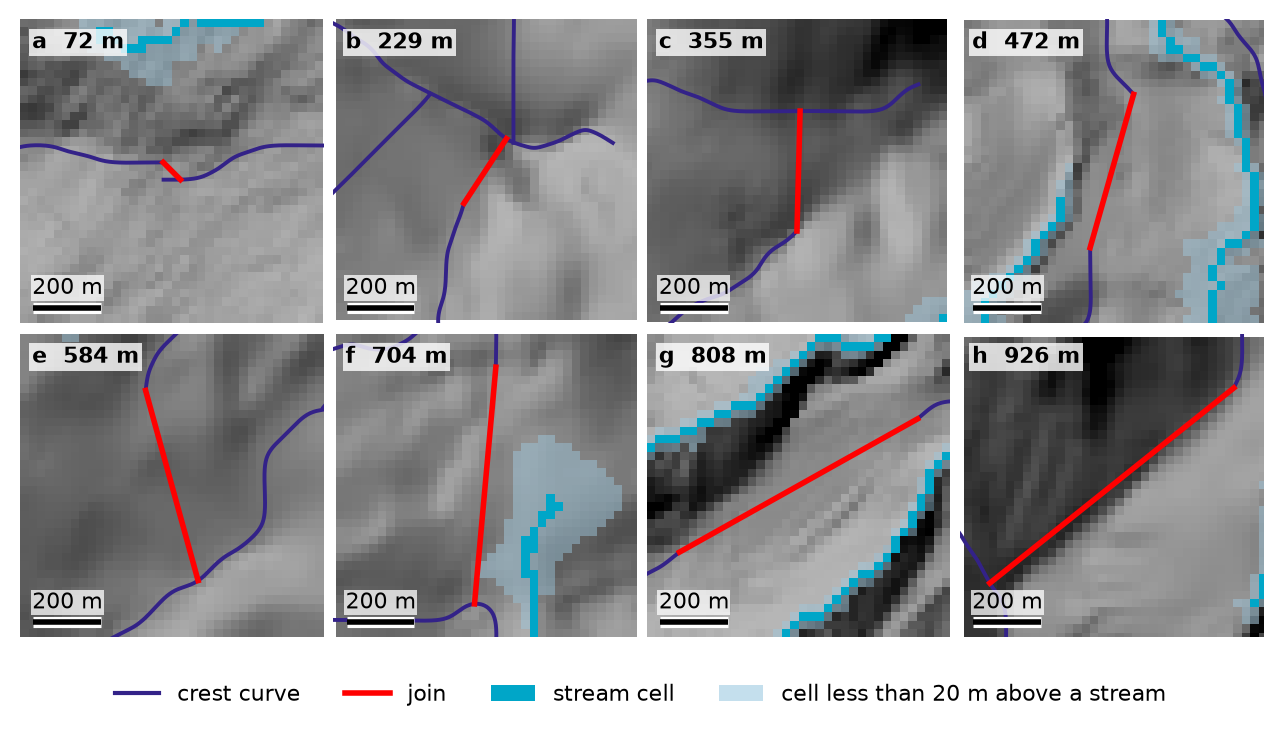
\includegraphics[width=0.9\textwidth]{figures/joins_alps.png}
\caption{A join is a short straight link between two crest curves that stays on the ridge. Eight joins of the Alps, from the shortest to the longest of the range, each in a window of the same size: the join (red), the crest curves,
the stream cells and the cells less than 20~m above a stream.}
\label{fig:joins}
\end{figure}

\section{Where the numbers hold}\label{app:limits}

Figure~\ref{fig:limits} shows the three limits of the exponent.

\begin{figure}
\centering
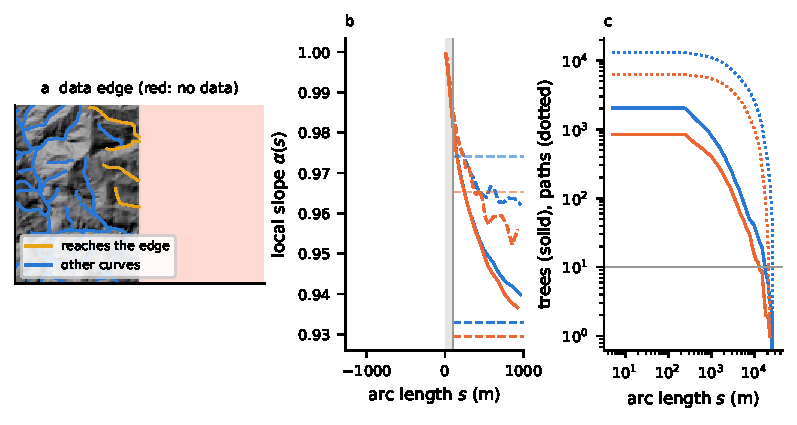
\includegraphics[width=0.9\textwidth]{figures/limits.pdf}
\caption{Three things limit the exponent: the data edge, the grid scale and the number of trees at long lags. \textbf{a}~The data edge where most flagged curves of the Alps are: pink, no elevation data; orange, curves that
reach the edge. \textbf{b}~Local slope of the MSD, $\alpha(s)$, near the grid scale; grey: below four cells. Dashed lines: $\Hgeo$ of the window from 0.1~km, as in Figure~\ref{fig:tamsd}b. \textbf{c}~Number of trees
(solid) and of paths (dotted) that reach each lag; the grey line is the minimum of \CgPMinCurves{} paths.}
\label{fig:limits}
\end{figure}

\paragraph{The data edge.} The model stops at the national border, which in the Pyrenees and in much of the Alps runs along the main divide, so a crest that reaches it is cut. \CgAlpsEdgeCurves{} Alps curves and
\CgPyrEdgeCurves{} Pyrenees curves are flagged, and so are \CgAlpsEdgePaths{} and \CgPyrEdgePaths{} paths. Table~\ref{tab:noedge} repeats the exponents without them; the point values of the paths are those of Table~\ref{tab:hgeo} to the third decimal, and only the ends of some intervals move in the last digit.

\paragraph{The grid scale.} Below four cells the divide runs on cell sides and the spline that smooths the steps makes the curve straighter than the terrain: $\alpha(s)$ is at least \CgGridAlphaMin{} there (panel b). The fit starts at
$\CgPFitFrom$~m and no window includes shorter lags.

\paragraph{Few trees at long lags.} A lag of 10~km needs a path of at least 40~km, since lags stop at a quarter of the path. Panel c shows how many trees carry each lag; the last window rests on \CgAlpsTreesTenKm{} trees in the Alps and
\CgPyrTreesTenKm{} in the Pyrenees, and a bootstrap that draws whole trees sees whether one of them is in or out. For the curves the population changes with the lag: only the longest curves reach large lags, so the mean at large $s$
is that of straighter curves and the local slope can exceed 1, as for the Alps curves between 1 and 10~km (\CgAlpsCurvesMid). That value measures the change of population, so the curves are used only below 1~km.

\begin{table}[H]
\centering
\caption{As Table~\ref{tab:hgeo} without the curves and paths that reach the edge of the data.}
\label{tab:noedge}
\small
\setlength{\tabcolsep}{4pt}
\begin{tabular}{lllll}
\toprule
 & \multicolumn{2}{c}{Alps} & \multicolumn{2}{c}{Pyrenees} \\
\cmidrule(lr){2-3}\cmidrule(lr){4-5}
window of $s$ & paths & curves & paths & curves \\
\midrule
from 0.1~km & 0.933 (0.928--0.940) & 0.974 (0.970--0.977) & 0.930 (0.925--0.933) & 0.965 (0.962--0.970) \\
0.1--1~km & 0.960 (0.959--0.961) & 0.971 (0.971--0.972) & 0.960 (0.959--0.962) & 0.969 (0.969--0.970) \\
1--10~km & 0.927 (0.921--0.934) & 1.004 (0.983--1.017) & 0.917 (0.912--0.922) & 0.967 (0.945--0.997) \\
beyond 10~km & 0.867 (0.814--0.934) & -- & 0.931 (0.773--0.977) & --
\\
\bottomrule
\end{tabular}
\end{table}

\section{Checks on the flights}\label{app:checks}

\subsection{Fixed windows of arc length}\label{sec:flwindows}

Does the picture of the rule change on fixed windows? Table~\ref{tab:flwindows} gives $H$ of the three curves on the windows of Table~\ref{tab:hgeo}, divided by $v$ to give lags. The window from 0.1~km starts at the floor and each curve
runs to its last lag with at least \flMinRows{} flights or paths, not to $\tau_b$. The order is that of the rule: the flights in time below the route and the route below the crests. The window beyond 10~km gives $H$ above 1 for the flights in time
and for the route. We attribute it to the selection of the longest flights at these lags, since only they reach them, and we do not interpret it.

\begin{table}[H]
\centering
\caption{$H$ on fixed windows of arc length $s = v\tau$, with 95\% intervals.}
\label{tab:flwindows}
\footnotesize
\setlength{\tabcolsep}{3pt}
\begin{tabular}{llccc}
\toprule
group & window of $s$ (km) & crests & flights in time & flights, route \\
\midrule
Alps, paragliders & from 0.1 & 0.935 (0.930--0.941) & 0.921 (0.917--0.923) & 0.943 (0.942--0.943) \\
Alps, paragliders & 0.1--1 & 0.961 (0.960--0.962) & 0.907 (0.907--0.908) & 0.937 (0.937--0.938) \\
Alps, paragliders & 1--10 & 0.927 (0.921--0.934) & 0.886 (0.885--0.887) & 0.918 (0.917--0.918) \\
Alps, paragliders & from 10 & 0.870 (0.814--0.938) & 1.059 (1.037--1.070) & 1.031 (1.024--1.038) \\
Pyrenees, paragliders & from 0.1 & 0.930 (0.927--0.935) & 0.898 (0.894--0.902) & 0.932 (0.930--0.935) \\
Pyrenees, paragliders & 0.1--1 & 0.960 (0.958--0.961) & 0.894 (0.892--0.896) & 0.937 (0.935--0.938) \\
Pyrenees, paragliders & 1--10 & 0.917 (0.912--0.923) & 0.871 (0.868--0.874) & 0.908 (0.906--0.911) \\
Pyrenees, paragliders & from 10 & 0.886 (0.775--0.958) & 1.031 (1.003--1.057) & 1.053 (1.031--1.075) \\
\bottomrule
\end{tabular}

\end{table}

\subsection{The flights alone from 10 s}\label{sec:flhten}

What is $H$ of the flights in time if the fit runs from 10~s to the last lag that at least ten flights reach? Table~\ref{tab:flhten} gives it with equal weight per flight and \flNBoot{} resamples of whole flights. It is higher
than the one of the rule (Table~\ref{tab:flh}), because only the longest flights reach the longest lags and $\alpha$ rises there (Figure~\ref{fig:routealpha}). It is therefore not the number compared with the crests.

\begin{table}[H]
\centering
\caption{$H$ of the flights in time fitted from 10~s to the last lag with at least ten flights, with 95\% intervals.}
\label{tab:flhten}
\small
\begin{tabular}{lrll}
\toprule
group & flights & $H$ & last lag (s) \\
\midrule
Alps, paragliders & 23320 & 0.926 (0.924--0.928) & 8537 \\
Pyrenees, paragliders & 2140 & 0.910 (0.904--0.914) & 6000 \\
\bottomrule
\end{tabular}

\end{table}

\subsection{Raw tracks and cleaned fixes}\label{sec:flraw}

Does the cleaning of the earlier analysis change $H$? The cleaning puts the fixes on a uniform time grid at the native cadence of the track (a shape-preserving cubic interpolation fills holes) and smooths east and north with a cubic
Savitzky--Golay filter whose timescale is 5~s and whose window has at least five samples; the filtered values replace the stored positions. On the sample run of \flRawNInSample{} paragliders, \flRawNBoth{} flights pass the selection from both
the raw IGC file (cut to the time in the air, spikes removed) and the cleaned fixes. The same resamples of flights give the difference of $H$ between the two, at $v = 35$~km/h (Table~\ref{tab:flrawcheck}). On the rule the difference raw
minus cleaned is \flRawDynRule{} for the flights in time (interval \flRawDynRuleLo{} to \flRawDynRuleHi) and \flRawRouteRule{} for the route (\flRawRouteRuleLo{} to \flRawRouteRuleHi). Both intervals contain zero: the cleaning does not change the
exponent within the interval of this sample, which is small.

\begin{table}[H]
\centering
\caption{$H$ of the same \flRawNBoth{} flights from the raw IGC files and from the cleaned fixes, and the difference, with 95\% intervals from the same resamples of flights.}
\label{tab:flrawcheck}
\footnotesize
\setlength{\tabcolsep}{3pt}
\begin{tabular}{llccc}
\toprule
curve & window of $s$ (km) & raw IGC & cleaned fixes & raw $-$ cleaned \\
\midrule
dyn & rule & 0.877 (0.865--0.888) & 0.885 (0.871--0.897) & $-$0.008 ($-$0.019 to 0.000) \\
dyn & 0.1-inf & 0.877 (0.865--0.889) & 0.887 (0.871--0.902) & $-$0.010 ($-$0.026 to 0.000) \\
dyn & 0.1-1 & 0.889 (0.879--0.898) & 0.890 (0.880--0.899) & $-$0.001 ($-$0.003 to 0.001) \\
dyn & 1-10 & 0.856 (0.840--0.870) & 0.867 (0.855--0.878) & $-$0.010 ($-$0.023 to $-$0.002) \\
dyn & 10-inf & 0.896 (0.802--0.969) & 0.963 (0.852--1.072) & $-$0.067 ($-$0.196 to 0.020) \\
route & rule & 0.921 (0.911--0.930) & 0.923 (0.913--0.932) & $-$0.002 ($-$0.006 to 0.000) \\
route & 0.1-inf & 0.921 (0.911--0.930) & 0.923 (0.912--0.932) & $-$0.002 ($-$0.006 to 0.001) \\
route & 0.1-1 & 0.934 (0.929--0.940) & 0.935 (0.929--0.940) & 0.000 ($-$0.001 to 0.000) \\
route & 1-10 & 0.914 (0.904--0.924) & 0.915 (0.905--0.924) & 0.000 ($-$0.004 to 0.002) \\
route & 10-inf & 0.917 (0.834--0.978) & 0.958 (0.880--1.020) & $-$0.041 ($-$0.103 to $-$0.004) \\
\bottomrule
\end{tabular}

\end{table}
